\documentclass[10pt,a4paper]{article}
\usepackage[utf8]{inputenc}
\usepackage[spanish, mexico]{babel}
\usepackage{listingsutf8}
\usepackage{color}
\usepackage{amsmath}
\usepackage{subfig}
\usepackage{graphicx}
\usepackage{multicol} 
\usepackage{float}
\usepackage{wasysym}
\definecolor{codegreen}{rgb}{0,0.6,0}
\definecolor{codegray}{rgb}{0.5,0.5,0.5}
\definecolor{codepurple}{rgb}{0.58,0,0.82}
\definecolor{backcolour}{rgb}{0.95,0.95,0.92}
\usepackage[top=2cm,bottom=3cm,left=3cm,right=3cm]{geometry}
\setlength{\parskip}{\baselineskip} 

\begin{document}

\setlength{\unitlength}{1cm}
\thispagestyle{empty}
\begin{picture}(18,4)
\put(0,0.2){
\includegraphics[scale=.2]{UNAM.jpg}}
\put(11.5,0){
\includegraphics[scale=.5]{fc.png}}
\end{picture}
\begin{center}
\textbf{{\LARGE Universidad Nacional Autónoma de México}\\[1cm]
{\LARGE Facultad de Ciencias}}\\[1.8cm]
{\LARGE Práctica 11: Velocidad del sonido en el aire y en $CO_2$  }\\[1.2cm]
\end{center}
\vspace{.7 cm}
\begin{flushleft}{\Large 31 de Octubre de 2019  }\\[0.6cm]
\end{flushleft}
\begin{flushright}{\Large{\underline{\textcolor{black}{López Cruz Ángel Jikmé}}}}\\[0.78cm]
\end{flushright}
\begin{flushright}{\Large{\underline{\textcolor{black}{López Velasco Juan Manuel}}}}\\[0.78cm]

\begin{flushright}{\Large{\underline{\textcolor{black}{Robledo Ibarra Emiliano}}}}\\[0.9cm]

\end{flushright}\end{flushright}
\begin{center}
{\Large Profesor: Luis Quintanar Robles }\\[0.8cm]
{\Large Ayudante: Luis Enrique Quintanar Cortés }\\[0.8cm]
\end{center}
RESUMEN:
La práctica tuvo como objetivo medir la velocidad del sonido en el aire y en dióxido de carbono, utilizando diferentes frecuencias y midiendo la longitud de onda apartir de los máximos obtenidos en el osciloscopio, es decir se graficó la longitud de onda obtenida y la inversa de la frecuencia, con lo que se obtuvo como pendiente la velocidad del sonido, el resultado fue el siguiente, en el aire de 345 $\pm$ 11 $\frac{m}{s}$ y en el $CO_2$ de 245 $\pm$ 8 $\frac{m}{s}$ además que por el coeficiente de determinación de nuestra recta asociada a la velocidad fue de 0.9928 y 0.975 respectivamente indicándonos una muy buena aproximación a la velocidad (pendiente) resultante, lo cual resalta una coherencia entre la relación entre estas dos variables.
\normalsize
\newpage


\section{Introducción}
El objetivo de la práctica fue medir la velocidad del sonido generado por un bocina en dos medios distintos: el aire de la CDMX y en $CO_2$. Para ello se aprovechó que el sonido se transmite por medio de ondas, pero para poder utilizar este hecho primero debemos saber qué es una onda y cómo podemos utilizar los parámetros que la caracterizan para poder medir la velocidad de la misma.

Una onda es una forma de propagación debida a la perturbación del medio donde esta se transmite. Hay distintos tipos de ondas que se clasifican respecto a su medio de propagación y también la forma en que se mueven. Debido a que es una forma natural de propagación se estudian varios aspectos de ellas: periodo ($T$), amplitud ($A$), frecuencia ($f$), fase ($\phi$), longitud de onda ($\lambda$), entre otros aspectos. Una característica muy importante de dicho fenómeno es que las ondas  se encuentran íntimamente relacionadas al hecho de que cuando hablamos de ellas, en realidad hablamos de la energía y una manera de transmisión. 

Las ondas pueden tener formas muy variadas, la más simple de ellas son las sinusoidales:

\begin{equation}
	f(x,t) = A sin (\omega t + kx) 
\end{equation}

Donde $A$ representa la amplitud de la onda, $\omega$ la frecuencia angular y $k$ el número de onda [1]. Tanto $\omega$ como $k$ al estar relacionados a un movimiento periódico cumplen dos relaciones: $\omega = 2\pi f$ y $k = \frac{2\pi}{\lambda}$. Además de que se pide que:

\begin{equation}
	v  = \frac{\omega}{k} = \frac{\lambda}{T} = \lambda f
\end{equation}

De aquí observamos que tanto la velocidad de la onda, la frecuencia y su longitud de onda están relacionadas, de esta manera si tenemos un sistema que evita el intercambio de materia (el gas donde se propagará el sonido) debería mantener la velocidad a la cual el sonido se propaga, por ello se propone usar un sistema cerrado para gases distintos al aire. Así que bajo la hipótesis de una onda descrita por una función seno es posible obtener la relación:

\begin{equation}
    \lambda = \frac{1}{f}v
\end{equation}

Que conociendo la longitud de onda y la frecuencia, se espera que se  relacionarían de manera lineal la frecuencia inversa y la longitud de onda donde la pendiente de la línea de ajuste entre estas dos variables resulta ser la velocidad de la onda. Para los valores teóricos de la velocidad del  sonido se encontró que en el $CO_2$ a 0ºC y a presión de una atmósfera es de  259 m/s [1] y que para el aire en condiciones de 20ºC a una atmósfera es de 344 m/s [2].



\section{Procedimiento.}
Se propuso un experimento en el cual se pudiese medir (medida directa) la longitud de una onda y la frecuencia de la misma para así poder calcular (medida indirecta) la velocidad de la onda en dos medios diferentes, los cuales fueron aire (la composición del aire de la CDMX) y $CO_2$.  

El sistema con el cual se midieron los parámetros antes mencionados consistió en un tubo cerrado con un pistón el cual en su interior contenía una bocina en uno de los extremos y un micrófono en el pistón. Un generador se conectaba a la bocina, con el cual se podía ajustar la frecuencia $f$ y la amplitud $A$ de la onda de sonido generada por la bocina. El micrófono se conectaba a un osciloscopio en el cual, ajustando correctamente todos los parámetros, se podía observar la representación de la onda generada por la bocina y captada por el micrófono. 

\begin{figure}[H]
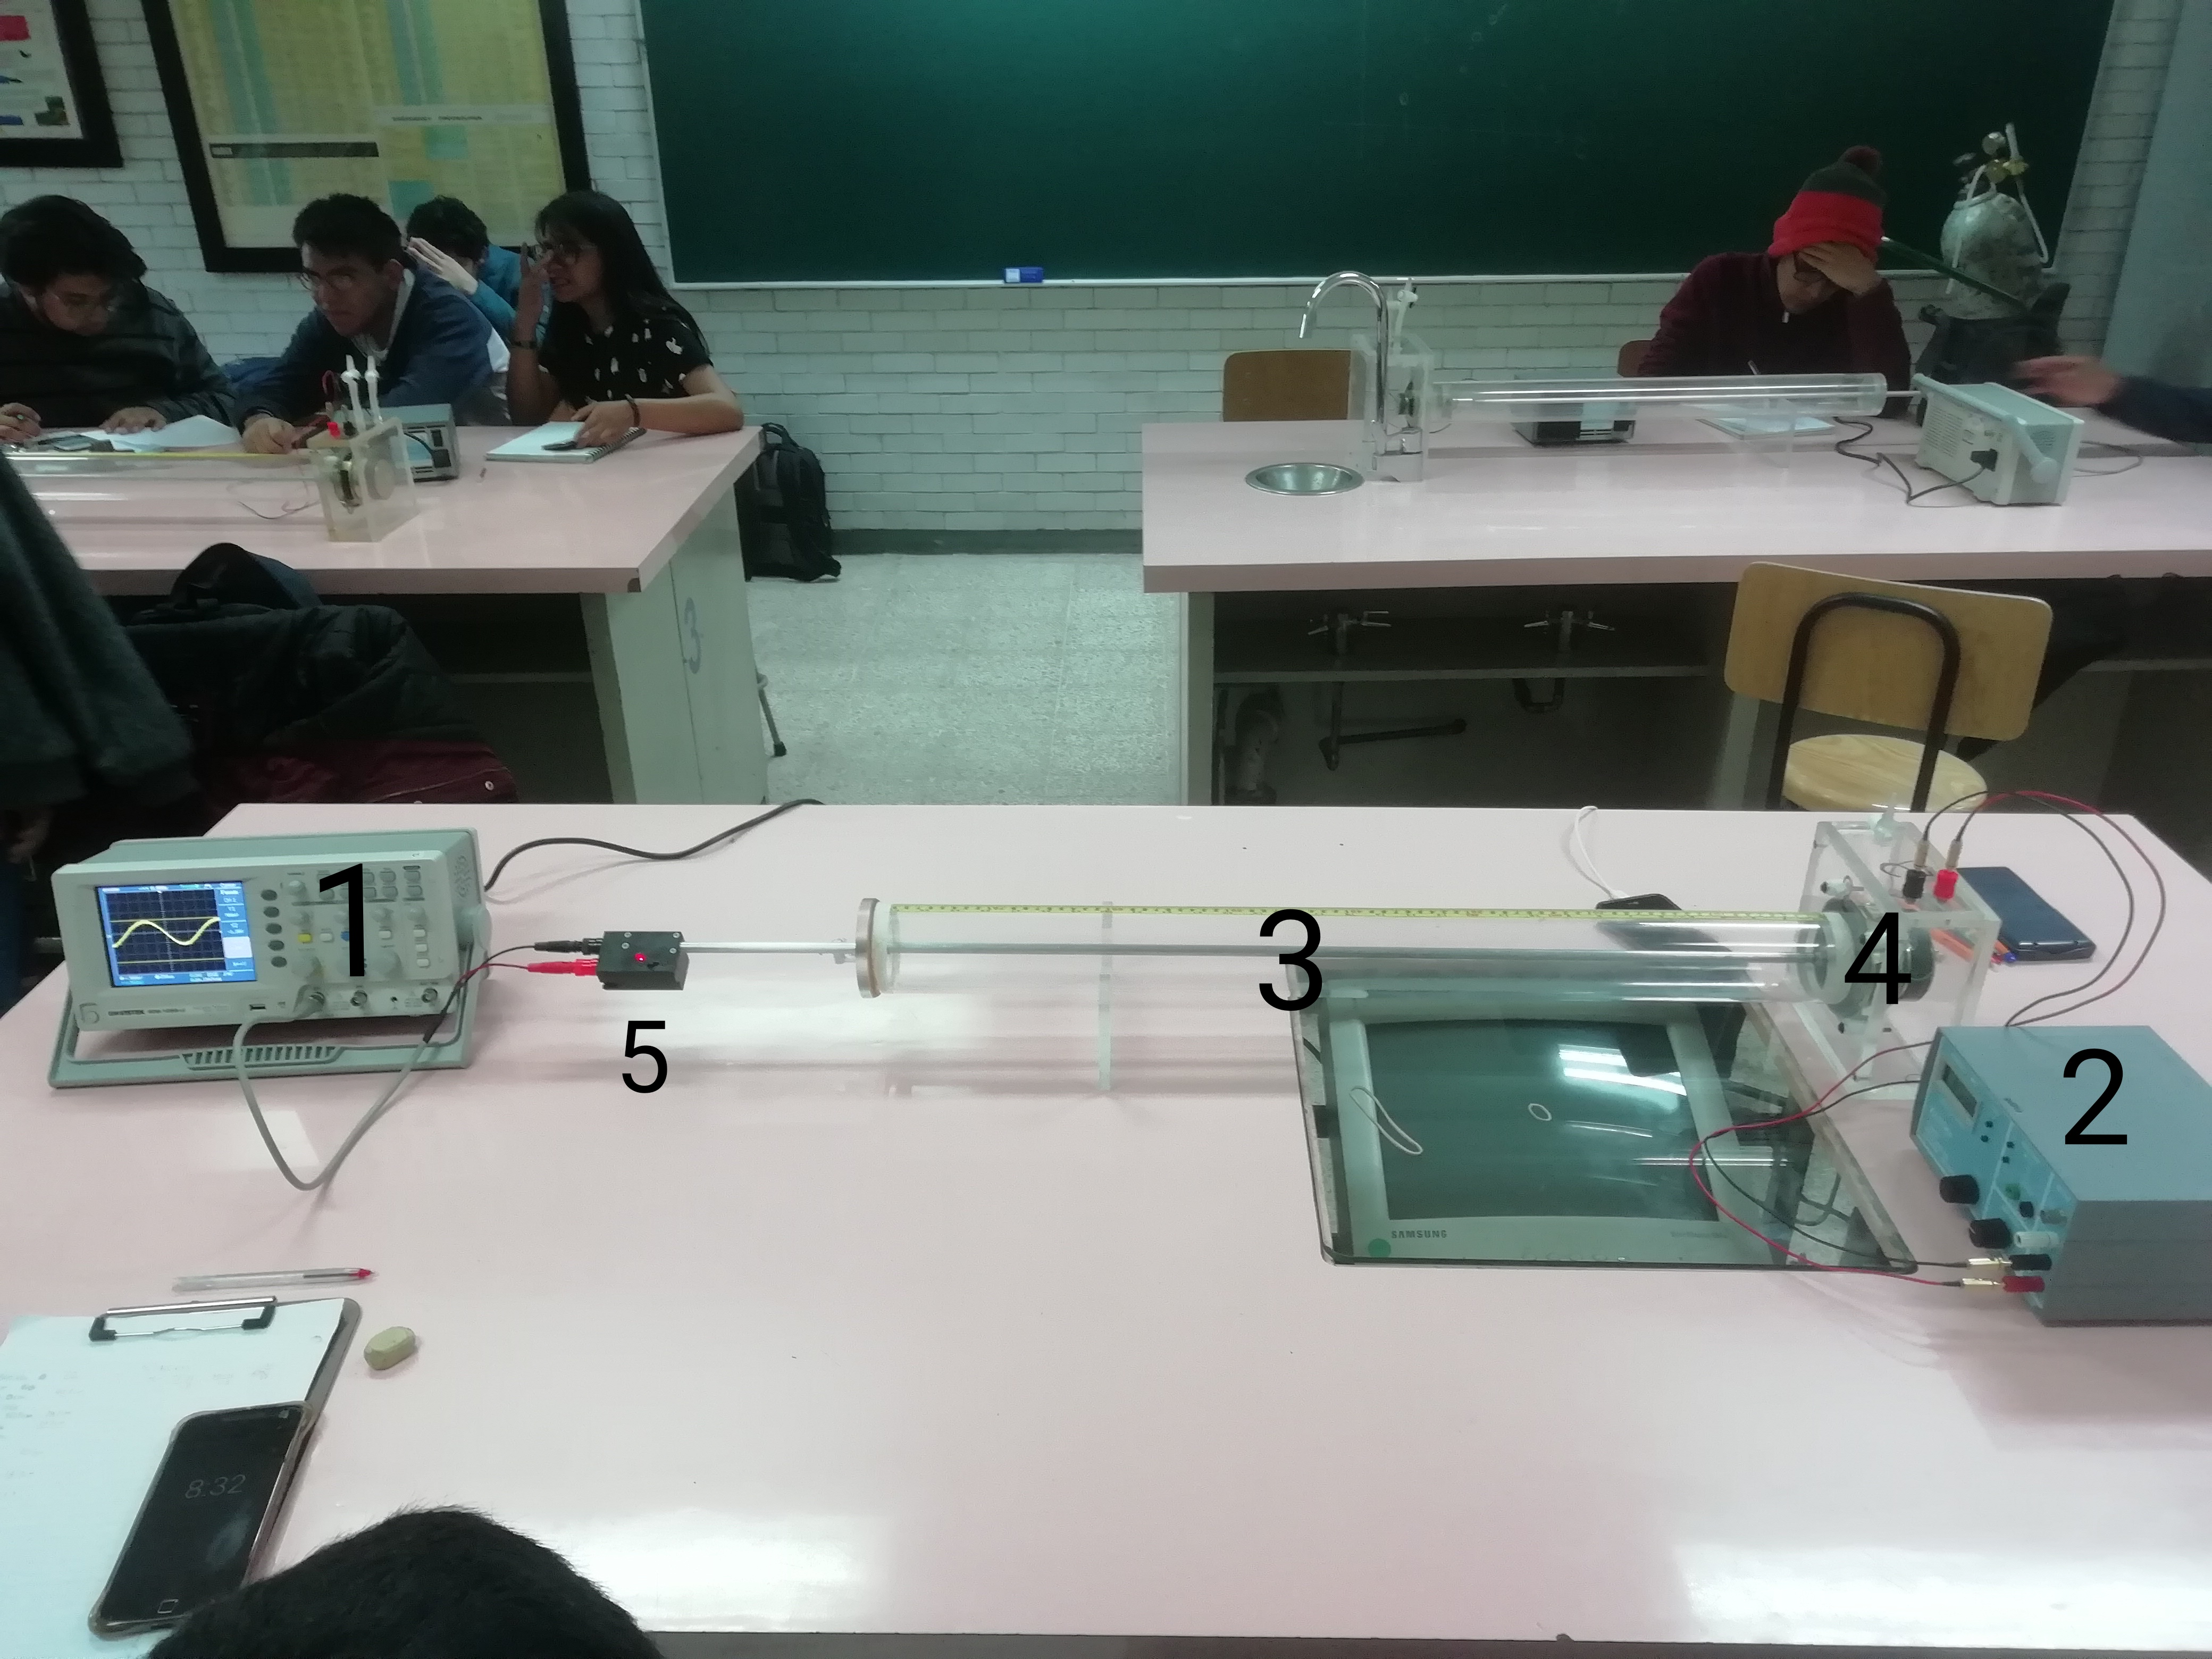
\includegraphics[scale=0.08]{esquema.jpg}
\centering
\caption{Diseño experimental: 1. Osciloscopio. 2. Generador. 3. Tubo cerrado, pistón y flexómetro. 4. Bocina. 5. Micrófono. }
\end{figure}

Dado que la longitud de una onda $\lambda$ es la distancia entre dos crestas o valles, para poder medirla se utilizó tanto el osciloscopio como el flexómetro colocado en el tubo; se deslizaba el pistón y se observaba la onda en la pantalla del osciloscopio y, dado que entre dos crestas (máximo alcance vertical de la onda) hay un valle (mínimo alcance vertical de la onda), se deslizaba el pistón hasta la posición en que se habían observado en la pantalla dos crestas (máximos) y un valle (mínimo). 
La frecuencia de la onda se ajustaba directamente con el generador. 
Se realizaron diez mediciones para el aire y diez mediciones para el $CO_2$, variando la frecuencia de la onda en cada una de ellas.  



\section{Resultados}
Se encontró que las mediciones de frecuencia y longitud de onda para ambos medios eran reproducibles. 

Tabla de datos del aire donde se muestra la longitud de onda $\lambda$ y la frecuencia de cada onda $f$ para cada medición.
\begin{table}[H]
  \centering
    \begin{tabular}{|c|c|c|} \hline
    Medición & Frecuencia $f$ [Hz] & Distancia $\lambda$ [m] \\ \hline
    1     & 450.0$\pm 0.5$ & 0.6180$\pm 0.0005$ \\ \hline
    2     & 500.0$\pm 0.5$ & 0.5300$\pm 0.0005$ \\ \hline
    3     & 550.0$\pm 0.5$ & 0.4400$\pm 0.0005$ \\ \hline
    4     & 600.0$\pm 0.5$ & 0.4070$\pm 0.0005$ \\ \hline
    5     & 650.0$\pm 0.5$ & 0.3600$\pm 0.0005$ \\ \hline
    6     & 666.0$\pm 0.5$ & 0.3420$\pm 0.0005$ \\ \hline
    7     & 700.0$\pm 0.5$ & 0.3240$\pm 0.0005$ \\ \hline
    8     & 750.0$\pm 0.5$ & 0.3000$\pm 0.0005$ \\ \hline
    9     & 800.0$\pm 0.5$ & 0.2660$\pm 0.0005$ \\ \hline
    10    & 850.0$\pm 0.5$ & 0.2430$\pm 0.0005$ \\ \hline
    \end{tabular}%
  \caption{Mediciones para la velocidad del sonido en el aire.}
\end{table}%




Tabla de datos del dióxido de carbono, en ella se muestra la longitud de onda $\lambda$ y la frecuencia de cada onda $f$ para cada medición.
\begin{table}[H]
  \centering
    \begin{tabular}{|c|c|c|} \hline
    Medición & Frecuencia $f$ [Hz] & Distancia $\lambda$ [m] \\ \hline
    1     & 300.00$\pm 0.05$ & 0.7250$\pm 0.0005$ \\ \hline
    2     & 450.00$\pm 0.05$ & 0.4350$\pm 0.0005$ \\ \hline
    3     & 500.00$\pm 0.05$ & 0.4020$\pm 0.0005$ \\ \hline
    4     & 550.00$\pm 0.05$ & 0.3440$\pm 0.0005$ \\ \hline
    5     & 600.00$\pm 0.05$ & 0.2820$\pm 0.0005$ \\ \hline
    6     & 650.00$\pm 0.05$ & 0.2760$\pm 0.0005$ \\ \hline
    7     & 666.00$\pm 0.05$ & 0.2650$\pm 0.0005$ \\ \hline
    8     & 700.00$\pm 0.05$ & 0.2470$\pm 0.0005$ \\ \hline
    9     & 750.00$\pm 0.05$ & 0.2330$\pm 0.0005$ \\ \hline
    10    & 800.00$\pm 0.05$ & 0.2030$\pm 0.0005$ \\ \hline
    11    & 850.00$\pm 0.05$ & 0.1890$\pm 0.0005$ \\ \hline
    \end{tabular}%
  \caption{Mediciones para la velocidad del sonido en $CO_2$}
\end{table}%

Luego de ello se calculó el inverso de la frecuencia y se graficó esta contra la longitud de onda. En este ajuste se obtuvieron dos pendientes: 

\begin{itemize}
    \item   La pendiente del aire: $345\pm11$.
    \item   La pendiente del $CO_2$: $245\pm8$.
    \item El coeficiente de determinación del aire: 0.9928
    \item El coeficiente de determinación del $CO_2$: 0.975
\end{itemize}

\begin{figure}[H]
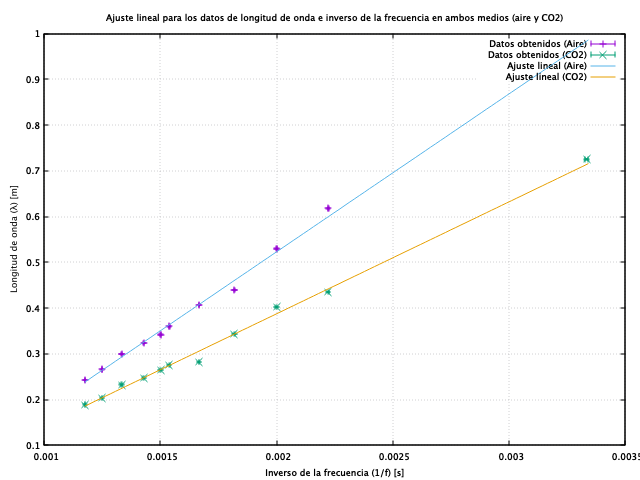
\includegraphics[scale=0.5]{AireyCO2.png}
\centering
\caption{Ajustes de rectas hechos a los datos del aire y $CO_2$.}
\end{figure}


\section{Análisis de resultados.}

De la ecuaciones planteadas en la introducción se puede concluir que la pendiente de las rectas obtenidas mediante el ajuste realizado de los datos experimentales del inverso de la frecuencia $1/f$ y la longitud de onda $\lambda$ representan la velocidad con la que la onda se propaga en el medio correspondiente (aire y $CO_2$). Haciendo el análisis dimensional se tiene que la velocidad $v$ de la onda tiene unidades de [m/s].

Así, la velocidad medida de una onda sonora en el aire fue $345 \pm 11$ m/s.

La velocidad medida para una onda sonora en $CO_2$ fue $245 \pm 8$ m/s.


\section{Conclusiones.}

Comparando las mediciones realizadas de la velocidad del sonido en el aire ($345 \pm 11$) m/s y en $CO_2$ ($245 \pm 8$ m/s) y los valores teóricos de dichas velocidades (344 m/s y 259 m/s, respectivamente) se tiene que el valor teórico de la velocidad del sonido en el aire se encuentra dentro del intervalo dado por el valor central de la medida y la incertidumbre asociada.

Para el valor medido de la velocidad del aire en el $CO_2$ se encontró que el valor teórico no estaba dentro del intervalo dado por el valor central de la medida y la incertidumbre asociada. Se tiene que el valor dentro del intervalo más próximo al valor teórico (253 m/s) difiere únicamente en un 2 $\%$ con respecto al valor teórico esperado. 

Como se ha visto, las propiedades de un gas dependen de las condiciones de presión y temperatura a la que se encuentren, por tanto, podemos concluir que dicha diferencia entre el valor medido experimentalmente y el valor teórico es debido a la diferencia en las condiciones de temperatura y presión con las que se realizó la medición (en el laboratorio la temperatura era de 21 grados Celsius a diferencia de los 0 grados Celsius con los que se obtuvo el dato teórico y la presión en la CDMX, a diferencia de la presión de 1 atm). Además de poder considerar dichos factores es también válido pensar en el sistema utilizado para medir y sus válvulas que no crean un sistema completamente perfecto y que debido a ello el gas dentro fue paulatinamente saliendo del sistema por lo cual no fue $CO_2$ puro, sin embargo la medición fue lo suficientemente cercana y los ajustes muy buenos de manera que podemos pensar en que se midió la velocidad del sonido para las condiciones de la CDMX a 21ºC. 




\begin{thebibliography}{a}
\bibitem{pradery} \textsc{Koshkin, N., \& Shirkévich, M.} (1975). \textit{Manual de Física}. (1st ed., p. 107). URSS: MIR.

\bibitem{pradery} \textsc{S.A.} (2003). \textit{PROPAGACIÓN DEL SONIDO}. Recuperado el 4 de Noviembre del 2019, de:  https://www.eumus.edu.uy/docentes/maggiolo/acuapu/prp.html.

\end{thebibliography}


\end{document}
